% 母子相似（射影定理）：Rt△ABC（∠C=90°），斜边 AB 上的高 CD
% 取 AC=3、BC=4、AB=5，D=A+0.36·(B-A)；得 AD=p=1.8、BD=q=3.2、CD=h=2.4
\documentclass[tikz,border=4pt]{standalone}
\usepackage{ctex}
\usepackage{amsmath}
\usetikzlibrary{calc}
\begin{document}
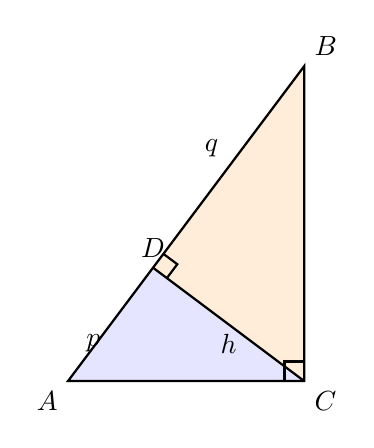
\begin{tikzpicture}[scale=1.0, thick]
  \coordinate (A) at (0, 0);
  \coordinate (C) at (3, 0);
  \coordinate (B) at (3, 4);
  \coordinate (D) at ($(A)!0.36!(B)$);

  % 两个小三角形浅填色
  \fill[blue!10]   (A) -- (C) -- (D) -- cycle;
  \fill[orange!15] (C) -- (B) -- (D) -- cycle;

  \draw (A) -- (B) -- (C) -- cycle;
  \draw (C) -- (D);

  % ∠C 直角符号
  \draw ($(C) + (-0.25, 0)$) -- ($(C) + (-0.25, 0.25)$) -- ($(C) + (0, 0.25)$);

  % ∠ADC 直角符号：AB 单位向量 (3/5, 4/5)，AB 法向（指向 C 一侧）(4/5, -3/5)
  \draw ($(D) + ({0.22*3/5}, {0.22*4/5})$)
     -- ($(D) + ({0.22*3/5 + 0.22*4/5}, {0.22*4/5 - 0.22*3/5})$)
     -- ($(D) + ({0.22*4/5}, {-0.22*3/5})$);

  \node[below left] at ($(A)!0.5!(D)$) {$p$};
  \node[above left] at ($(D)!0.5!(B)$) {$q$};
  \node[below]      at ($(C)!0.5!(D)$) {$h$};

  \node[below left]  at (A) {$A$};
  \node[above right] at (B) {$B$};
  \node[below right] at (C) {$C$};
  \node[above]       at (D) {$D$};
\end{tikzpicture}
\end{document}
